\chapter{Raízes unitárias, regressão espúria e cointegração}
\label{cap:ur}

\section{Tendência determinística versus estocástica}
Duas séries podem ``subir'' por motivos muito diferentes.
\begin{itemize}[leftmargin=1.4em]
\item \textbf{Tendência determinística}: $y_t=a+bt+\text{(estacionário)}$. Os desvios da reta são temporários. Remover a tendência torna a série estacionária.
\item \textbf{Tendência estocástica} (raiz unitária): $y_t=y_{t-1}+\varepsilon_t$. Os choques são permanentes. Remover uma reta \emph{não} resolve; é preciso diferenciar.
\end{itemize}
Tratar uma como se fosse a outra gera erros graves de previsão e de inferência.

\section{Teste de Dickey--Fuller aumentado (ADF)}
Estima-se
\[
\Delta y_t=\alpha+\gamma\,y_{t-1}+\sum_{j=1}^{p}\delta_j\Delta y_{t-j}+e_t,
\]
e testa-se $H_0:\gamma=0$ (há raiz unitária) contra $\gamma<0$ (estacionária). As defasagens extras servem para branquear os resíduos.

\begin{atencao}[{Armadilhas do ADF}]
\begin{itemize}[leftmargin=1.2em]
\item \textbf{A estatística t não segue a distribuição t nem a normal}. Os valores críticos são os de Dickey--Fuller, mais negativos (por exemplo, cerca de $-2{,}86$ a 5\% com constante). Comparar com $-1{,}96$ rejeita demais.
\item \textbf{Os termos determinísticos importam}: sem constante, com constante ou com tendência, os valores críticos mudam e a escolha errada distorce o teste.
\item \textbf{Baixo poder}: o teste tem dificuldade em distinguir raiz unitária de uma raiz próxima de 1 (por exemplo, $\phi=0{,}98$) em amostras moderadas.
\item \textbf{KPSS inverte a hipótese nula} (a nula é estacionariedade). Usar os dois juntos é prática comum: ADF rejeita e KPSS não rejeita $\Rightarrow$ evidência favorável à estacionariedade.
\end{itemize}
\end{atencao}

\begin{simulacao}[{Conferido por simulação}]
Num passeio aleatório de 300 pontos, o ADF deu p-valor $0{,}50$ (não rejeita a raiz unitária, correto). Num ruído branco, o p-valor foi $\approx10^{-29}$ (rejeita fortemente, correto).
\end{simulacao}

\section{Regressão espúria}
Regredir uma série integrada contra outra, independente dela, produz coeficientes ``significativos'' com frequência absurda.

\begin{simulacao}[{Conferido por simulação}]
Simulei 1000 pares de passeios aleatórios \emph{independentes} com 200 observações cada, rodei MQO de um contra o outro e testei a inclinação a 5\%. O teste t rejeitou a hipótese de inclinação zero em \textbf{83,6\%} dos casos, em vez dos 5\% esperados.
\end{simulacao}

\begin{center}
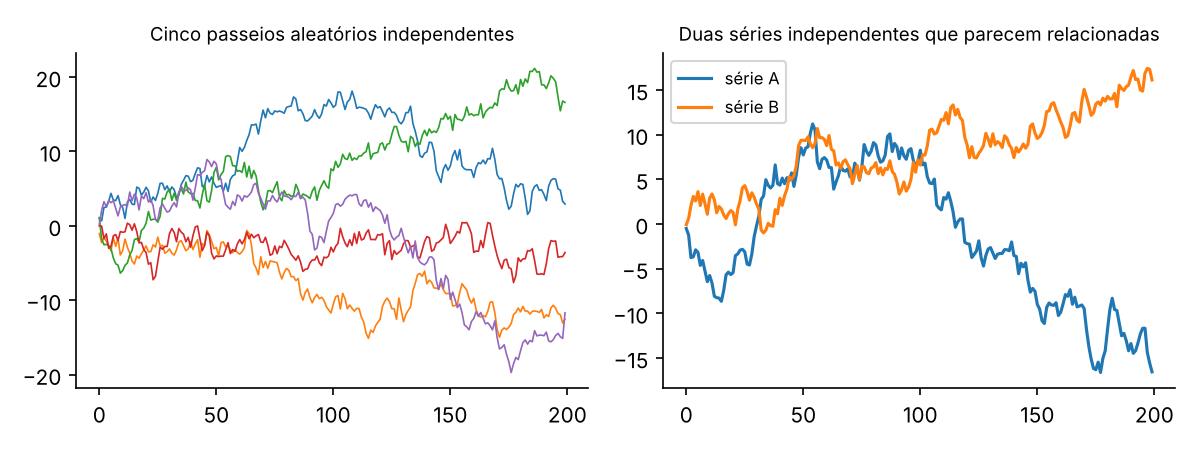
\includegraphics[width=0.9\textwidth]{fig/espuria.png}\\
\small Esquerda: cinco passeios aleatórios independentes, que parecem ter tendências próprias. Direita: duas séries independentes que, por acaso, parecem relacionadas.
\end{center}

\textbf{Regras práticas}: (i) nunca faça MQO em níveis de séries com raiz unitária sem investigar cointegração; (ii) um sinal de alerta clássico é $R^2$ alto com resíduos fortemente autocorrelacionados (estatística de Durbin--Watson próxima de 0); (iii) se não há cointegração, trabalhe com as séries diferenciadas.

\section{Cointegração}
Duas séries $I(1)$ são \textbf{cointegradas} se alguma combinação linear delas é estacionária. Elas podem se afastar no curto prazo, mas uma força as traz de volta (um equilíbrio de longo prazo).

\begin{intuicao}[{O bêbado e o cachorro}]
Dois passeios aleatórios independentes são como um bêbado e um cachorro soltos: cada um vai para onde quer. Cointegração é o bêbado com o cachorro na coleira: ambos vagam sem rumo, mas a distância entre eles é limitada.
\end{intuicao}

\begin{center}
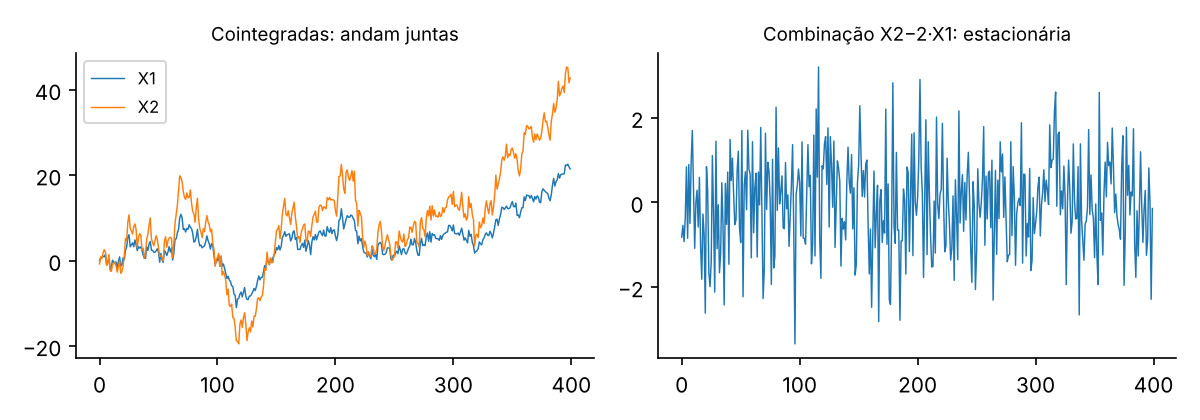
\includegraphics[width=0.9\textwidth]{fig/cointegracao.png}\\
\small $X_1=w+\text{ruído}$ e $X_2=2w+\text{ruído}$, com $w$ um passeio aleatório. Cada série é não estacionária, mas $X_2-2X_1$ é estacionária.
\end{center}

\textbf{Teste de Engle--Granger} (dois passos): (1) regrida uma série na outra; (2) aplique ADF aos resíduos, usando valores críticos \emph{próprios} para resíduos estimados (mais exigentes que os do ADF comum). A alternativa multivariada é o teste de Johansen, que identifica quantas relações de cointegração existem.

\begin{simulacao}[{Conferido por simulação}]
Com 200 observações, repeti 500 vezes. Para pares cointegrados, o teste de Engle--Granger a 5\% rejeitou ``sem cointegração'' em 99,6\% das simulações. Para pares independentes, rejeitou em 7,4\% (um pouco acima dos 5\% nominais em amostras de tamanho moderado, mas muito longe de 84\%).
\end{simulacao}

\textbf{Modelo de correção de erros}: se $y_t$ e $x_t$ são cointegradas, $\Delta y_t=\alpha(y_{t-1}-\beta x_{t-1})+\gamma\Delta x_t+e_t$, com $\alpha<0$ medindo a velocidade com que a economia retorna ao equilíbrio.

\begin{exercicio}
Uma regressão entre duas séries de preços em nível dá $R^2=0{,}95$ e Durbin--Watson de $0{,}1$. O que fazer antes de confiar nesse resultado?
\end{exercicio}
\sol{O padrão ($R^2$ alto, DW muito baixo) é típico de regressão espúria. Teste raiz unitária em cada série; se ambas forem $I(1)$, teste cointegração (Engle--Granger ou Johansen). Sem cointegração, a regressão em níveis não tem interpretação e o correto é modelar as diferenças. Com cointegração, use um modelo de correção de erros.}
